%!TEX TS-program = xelatex
%!TEX encoding = UTF-8 Unicode

%%%  Syllabus template for use with style files at http://kjhealy.github.com/latex-custom-kjh
%%%  Kieran Healy

\documentclass[11pt,article,oneside]{memoir}

% packages
\usepackage{org-preamble-xelatex} 

\AtBeginBibliography{\small}

% Definitions
\def\myauthor{Author}
\def\mytitle{Title}
\def\mycopyright{\myauthor}
\def\mykeywords{}
\def\mybibliostyle{plain}
\def\mybibliocommand{}
\def\mysubtitle{}
\def\myaffiliation{Louisiana State University}
\def\myaddress{100 Design}
\def\myemail{baharmon@lsu.edu} %harmon1@lsu.edu
\def\myweb{https://baharmon.github.io/}
\def\myphone{919.622.8414}
\def\myversion{}
\def\myrevision{}
\def\myaffiliation{\ \\Louisiana State University}
\def\myauthor{Brendan Harmon}
\def\mykeywords{Landscape Architecture, Syllabus, Graduate}
\def\mysubtitle{Syllabus}
\def\mytitle{{\normalsize \textsc{LA} 3001\newline} \huge \bfseries 
Ecological Restoration Studio}

\begin{document}

\setlength\bibitemsep{0.75em}

% fonts
\defaultfontfeatures{}
\defaultfontfeatures{Scale=MatchLowercase}         
\setmainfont[Scale=1, Path = fonts/lato/,BoldItalicFont=Lato-RegIta,BoldFont=Lato-Reg,ItalicFont=Lato-LigIta]{Lato-Lig}
\setsansfont[Scale=1, Path = fonts/lato/,BoldItalicFont=Lato-RegIta,BoldFont=Lato-Reg,ItalicFont=Lato-LigIta]{Lato-Lig}
\setmonofont[Mapping=tex-text,Scale=0.8,Path = fonts/inconsolata/]{i}

\def\ind{\hangindent=1 true cm\hangafter=1 \noindent}
\def\labelitemi{$\cdot$}
\chapterstyle{article-4-sans}  
\title{\LARGE \mytitle}     
\author{\Large\myauthor \newline \footnotesize\texttt{\noindent\myemail}}
\date{Fall 2017. Design 217.\newline Monday, Wednesday, \& Friday 1:30am--5:20pm.}
\published{\,}

\maketitle

% -------------------------------- COVER PAGE -------------------------------- 

% full page image with no borders, 30% opacity, greyscale
% image: orthoimagery | flooded elevation 

% -------------------------------- DESCRIPTION -------------------------------- 

\section{Course Description}

In this studio you will plan and design the restoration 
of the Golden Meadows coastal wetland. 
%
You will conduct research and develop designs 
across spatial and temporal scales.
%
First you will map and model landscape patterns and processes 
at regional to site scales using geographic information systems (GIS) 
and digital illustration. 
Then you will develop a masterplan for the region based on
shifting ecological baselines and suitability analysis.
Finally you will design the wetland park and reserve
with a phased planting plan that will evolve over time. 
%
This course will introduce you to the basics of cartography, 
geospatial analysis and modeling, digital fabrication,
and rapid ideation.
You will use both analog and digital media including
freehand drawing, GIS, 3D modeling, 
and computer numerical controlled (CNC) milling.
%\\
%\noindent \textbf{Format}
Generally on Tuesdays there will be a workshop or seminar
and on Thursdays there will be desk critiques, pinups, or reviews. 
There will also be a site visit 
and a couple of workshops on special topics on Saturdays.\\

%\begin{figure}
%    \begin{center}
%        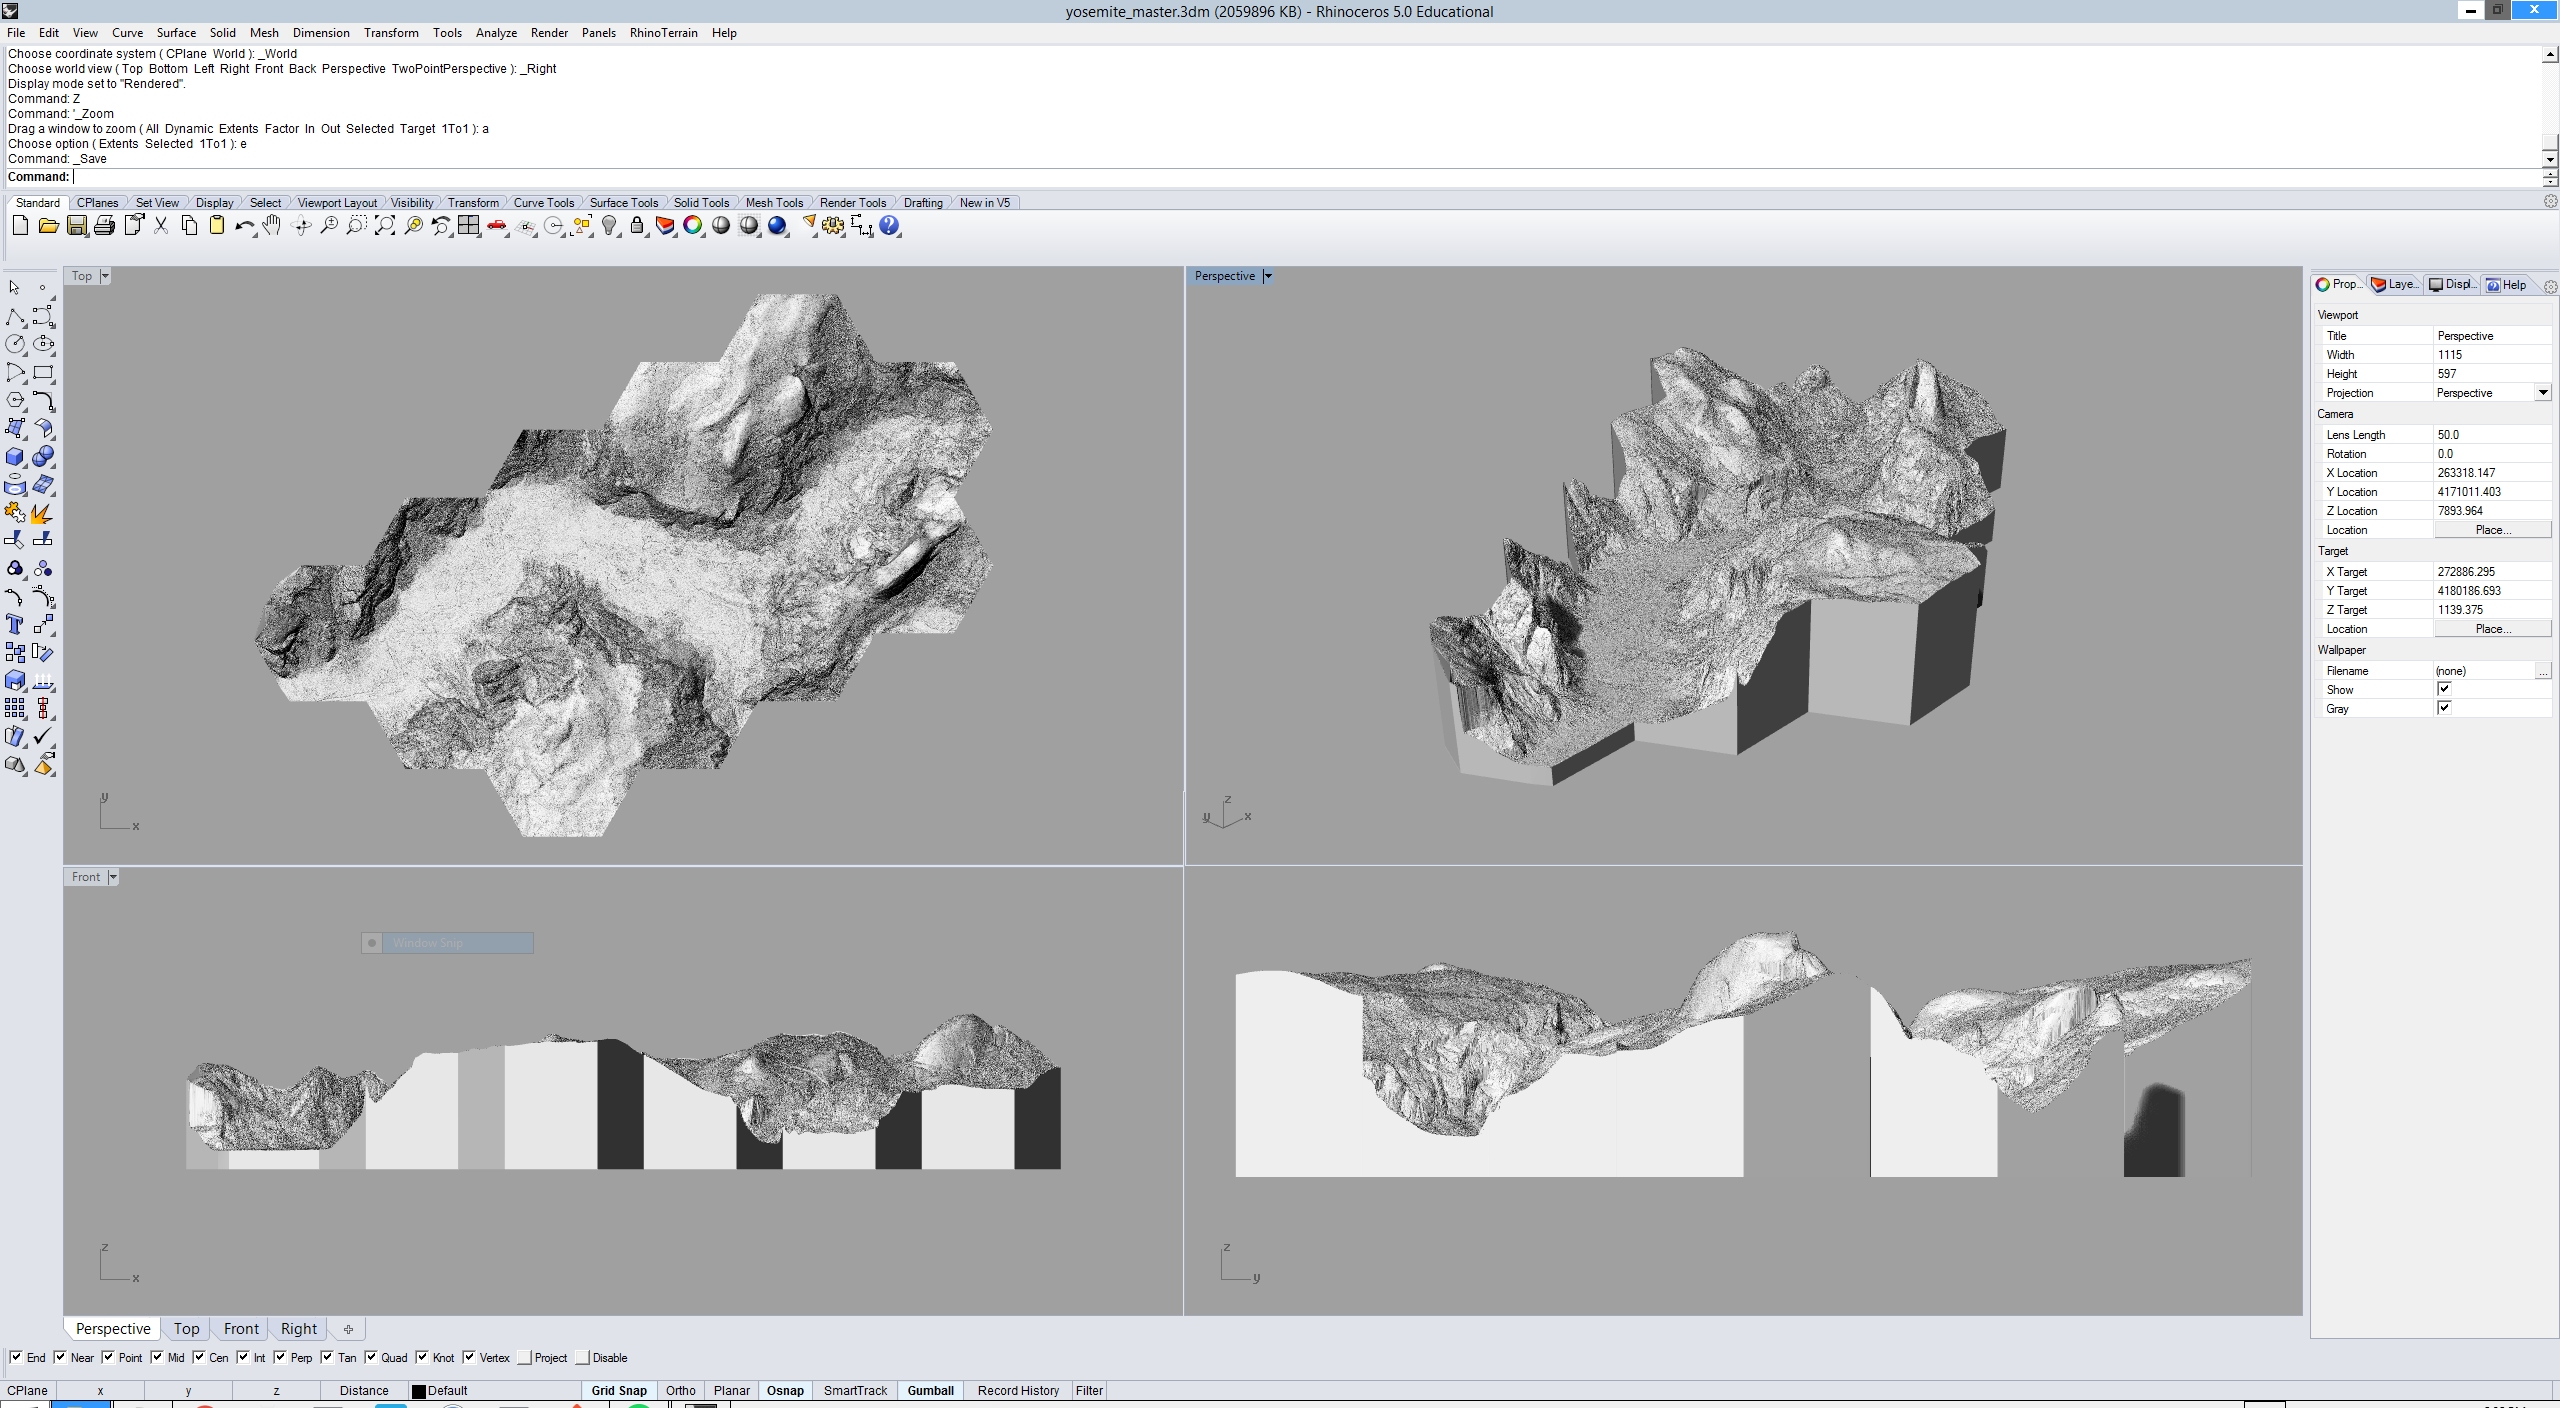
\includegraphics[width=\textwidth]{images/yosemite_1.png}
%        \caption{...}
%        \label{fig:yosemite}
%    \end{center}
%\end{figure}

\clearpage

% -------------------------------- SCHEDULE -------------------------------- 
\section{Course Schedule}

\begin{table}[H]
\small
\begin{tabular}{l l @{\hskip 1cm}l}
%
\textbf{1} & Design charrette\\
\textbf{2} & Field trip\\
\textbf{3} & Precedent studies\\
\textbf{4} & Cartography & \textbf{Site visit:} Golden Meadows\\
\textbf{5} & Topography\\
\textbf{6} & Hydrology\\
\textbf{7} & Ecosystems & \textbf{Review:} Maps\\ %
\textbf{8} & Ecological baselines & \textbf{Workshop:} Digital fabrication\\
\textbf{9} & Suitability analysis\\
\textbf{10} & Trail planning\\
\textbf{11} & Masterplanning & \textbf{Review:} Masterplan\\ %
\textbf{12} & Site design\\
\textbf{13} & Trail design & \textbf{Workshop:} Drawing\\
\textbf{14} & Planting design\\
\textbf{15} & Phased planting design & \textbf{Final review:} Site design\\ %
%
\end{tabular}
\end{table}

%\clearpage

% -------------------------------- PROJECTS -------------------------------- 
\section{Projects}
\renewcommand*{\bibfont}{\footnotesize}

You will work in small teams 
and submit a digital collection of your design work
at the final review. \\

\noindent \textbf{Mapping}
Your team will use GIS to map, analyze, and simulate 
the physical patterns and processes that shape
the Bayou La Fourche watershed. 
At the review your team will present
maps of infrastructure, topography, hydrology, and ecosystems
representing each of these systems at a range of scales. 
\\

\noindent \textbf{Masterplanning}
Your team will develop a GIS-based masterplan for the region 
using map overlay, suitability, and least cost path analysis. 
At the review your team will present
an illustrative masterplan, concept diagrams,
and a physical model of the landscape.
\\

\noindent \textbf{Site design}
Your team will develop a site design
addressing program, trails, and planting
for the restored wetland.
At the final review your team will present
a site plan, a series of phased planting plans,
sections, and a perspective.
\\

%\clearpage

% -------------------------------- SESSIONS -------------------------------- 
\section{Sessions}

\noindent \textbf{Design charrette}
A design charrette for the Louisiana Governor's Mansion.\\

\noindent \textbf{Field trip}
We will visit Washington DC and New York City. 
In Washington DC we will explore traces of the L'Enfant plan
and tour the city's museums and monuments.
In New York City we will visit design firms including 
MVVA, SCAPE, and Robert A.M. Stern Architects  
and tour projects like the Brooklyn Bridge Park and the High Line.
We will also learn about 
US Army Corps of Engineers' coastal resilience projects
and tour their projects on the New Jersey shore.\\

\noindent \textbf{Precedent studies}
In groups you will study one of the following projects:\\

\noindent
Louisiana Coastal Masterplan | \url{http://coastal.la.gov/2017-coastal-master-plan/}\\
Netherlands National Coastal Strategy | \\
\url{http://rijksoverheid.minienm.nl/nvk/NationalCoastalStrategy.pdf}\\
The Sand Engine | \url{http://www.dezandmotor.nl/en/}\\
Delta Works | \url{http://www.deltawerken.com/}\\
% https://deltaprogramma2017.deltacommissaris.nl/
% http://rijksoverheid.minienm.nl/nvk/NationalCoastalStrategy.pdf
MOSE | \url{https://www.mosevenezia.eu/}\\
Oystertecture | \url{http://www.scapestudio.com/projects/oyster-tecture/}\\
New Meadowlands | \url{http://newmeadowlands.org/}\\
Fresh Kills | \url{http://freshkillspark.org/}\\
% Fresh Kills Competition: http://www1.nyc.gov/assets/planning/download/pdf/plans/fkl/fkl.pdf
% Fresh Kills Masterplan: http://freshkillspark.org/wp-content/uploads/2013/07/Fresh-Kills-Park-Draft-Master-Plan.pdf

\noindent \textbf{Cartography}
An introduction to GIS and mapping. 
You will learn how to acquire geospatial data and elegantly map it.
You will produce a series of infrastructural maps of the study region. 
% Examples: http://atlas-for-the-end-of-the-world.com/world_maps_main.html
%
\nocite{*} \printbibliography[keyword=cartography, heading=none]
\vspace*{0.5em}

\noindent \textbf{Topography} 
You will acquire elevation data, 
model topography as digital elevation models in GIS 
and meshes in Rhino,
and analyze topographic parameters 
such as contours, slope, hillshading, and landforms.
You will also visualize topography and sunlight in 3D using Rhino.
You will produce a series of topographic maps 
and perspective renderings of the study region.\\

\noindent \textbf{Hydrology} 
You will model watersheds and water accumulation 
and simulate water flow, sediment flux, and flooding. 
You will produce a series of hydrological maps of the study region.\\

\noindent \textbf{Ecosystems}
You will derive high resolution landcover 
from orthophotography using image classification, 
analyze habitat fragmentation, and map ecosystem diversity.
You will produce a series of ecosystem maps of the study region.\\

\noindent \textbf{Ecological baselines}
%Ecological baseline seminar
	%Readings: rewilding, etc
%Digital fabrication workshop
	%Resources: 
%Ecological baseline charrette
\\
%
\nocite{*} \printbibliography[keyword=baselines, heading=none]
\vspace*{0.5em}

\noindent \textbf{Suitability analysis}
%
\nocite{*} \printbibliography[keyword=suitability, heading=none]
\vspace*{0.5em}

\noindent \textbf{Trail planning}
\\

\noindent \textbf{Masterplanning}
% Review: Masterplan\\
\\

\noindent \textbf{Site design}
\\

\noindent \textbf{Trail design}
% Drawing workshop
\\

\noindent \textbf{Planting design}
%
% 
% Reading: Piet Oudlof, Planting: A New Perspective
\nocite{*} \printbibliography[keyword=planting, heading=none]
\vspace*{0.5em}

\noindent \textbf{Phased planting design}
%Final review
\\

\clearpage

% -------------------------------- Supplies --------------------------------  
\section{Supplies}
Alcohol-based markers | \emph{Chartpak or Copic}\\
Felt-tip markers | \emph{Tombow Dual Brush Pens or Pentel Sign Pen}\\
Trace | \emph{White or Canary}\\
Polymer enriched sand | \emph{Kinetic Sand, 11~lbs}\\
Medium density fiberboard \\

% -------------------------------- Software -------------------------------- 
\section{Software}
GRASS GIS | \url{https://grass.osgeo.org/}\\
QGIS | \url{https://www.qgis.org/}\\
ArcGIS | \url{http://www.esri.com/arcgis/about-arcgis/}\\
Rhinoceros | \url{https://www.rhino3d.com/}\\
RhinoTerrain | \url{http://www.rhinoterrain.com/}\\
RhinoCAM | \url{https://mecsoft.com/rhinocam-software/}\\
Adobe Creative Cloud | \url{http://www.adobe.com/creativecloud.html}\\

% -------------------------------- Resources -------------------------------- 
\section{Resources}
Intro to GRASS GIS | \url{https://ncsu-geoforall-lab.github.io/grass-intro-workshop/}\\
Hydrology in GRASS GIS | \url{https://grasswiki.osgeo.org/wiki/Hydrological_Sciences}\\

\clearpage
% -------------------------------- Readings -------------------------------- 
\section{Readings}
\renewcommand*{\bibfont}{\normalsize} %\small
\vspace*{0.5cm}
\nocite{*}
\setlength\bibitemsep{1\baselineskip}
\printbibliography[heading=none]

\clearpage

% -------------------------------- Policies -------------------------------- 
\section{Policies}

\noindent \textbf{Time Commitment Expectations}
LSU's general policy states that for each credit hour, you (the student) should plan to
spend at least two hours working on course related activities outside of class. Since this course is for three credit hours, you should expect to spend a minimum of six hours outside of class each week working on assignments for this course. For more information see: 
\url{http://catalog.lsu.edu/content.php?catoid=12&navoid=822}.\\

\noindent \textbf{LSU student code of conduct}
The LSU student code of conduct explains student rights, excused absences, and what is expected of student behavior. Students are expected to understand this code:  \url{http://students.lsu.edu/saa/students/code}.\\ %Any violations of the LSU student code will be duly reported to the Dean of Students.\\

\noindent \textbf{Disability Code}
The University is committed to making reasonable efforts to assist individuals with disabilities in
their efforts to avail themselves of services and programs offered by the University. To this end,
Louisiana State University will provide reasonable accommodations for persons with
documented qualifying disabilities. If you have a disability and feel you need accommodations in
this course, you must present a letter to me from Disability Services in 115 Johnston Hall,
indicating the existence of a disability and the suggested accommodations.\\

\noindent \textbf{Academic Integrity}
According to section 10.1 of the LSU Code of Student Conduct, ``A student may be charged with Academic Misconduct'' for a variety of offenses, including the following: unauthorized copying, collusion, or collaboration; ``falsifying'' data or citations; ``assisting someone in the commission or attempted commission of an offense''; and plagiarism, which is defined in section 10.1.H as a ``lack of appropriate citation, or the unacknowledged inclusion of someone else's words, structure, ideas, or data; failure to identify a source, or the submission of essentially the same work for two assignments without permission of the instructor(s).''\\

\noindent \textbf{Plagiarism and Citation Method}
Plagiarism is the ``lack of appropriate citation, or the unacknowledged inclusion of someone else's words, structure, ideas, or data; failure to identify a source, or the submission of essentially the same work for two assignments without permission of the instructor(s)'' (Sec. 10.1.H of the LSU Code of Student Conduct). As a student at LSU, it is your responsibility to refrain from plagiarizing the academic property of another and to utilize appropriate citation method for all coursework. In this class, it is recommended that you use Chicago Style author-date citations. Ignorance of the citation method is not an excuse for academic misconduct. 

\end{document}
